\documentclass{article}
\usepackage[utf8]{inputenc}
\usepackage{fontspec}
\usepackage{natbib}
\usepackage{graphicx}
\usepackage{booktabs}
\usepackage{array}
\usepackage{multirow}
\usepackage[margin=0.8in]{geometry}
\usepackage[hidelinks]{hyperref}

% Compile with XeLaTeX (not pdfLaTeX) -- required for the inline Hebrew
% examples below. On Overleaf: Menu -> Compiler -> XeLaTeX.
\newfontfamily\hebrewfont{DejaVu Sans}
\newcommand{\heb}[1]{{\hebrewfont #1}}

\title{Repairing the Negation Blind Spot in Hebrew Text Embeddings}
\author{Itay Boros (ID.\ 211869987), Shachar Ben Zur (ID.\ 212373005)}
\date{Submitted as final project report for the NLP course, Reichman University, 2026}

\begin{document}
\maketitle

\begin{abstract}
Sentence embedding models are widely assumed to be sensitive to meaning, but
negation is a direct test of that assumption: a sentence and its negation
share nearly every surface word while meaning the opposite thing. We
measure this \emph{negation blind spot} in four frozen Hebrew-capable
embedders using a hand-verified probe mined from HebNLI (303 triples), and
find it real: two of four models score a sentence's negation as more
similar to it than a faithful paraphrase. We test two post-hoc repairs.
\texttt{projection} amplifies each sentence's own component along an
estimated negation direction in the frozen embedding space; naively
selecting its amplification strength by the headline metric alone
collapses the representation (unrelated sentences become near-identical,
$\mathrm{sim\_unrelated}{=}0.975$) rather than fixing it, and only a
second, independent guard metric catches this. \texttt{nli\_rerank} instead
blends the frozen cosine with a decontaminated, task-specific Hebrew NLI
classifier under a principled selection rule for the blend weight, reaching
$\geq$0.986 pairwise accuracy on every model. The paper's contribution is
less the two fixes themselves than the shared methodological finding
behind them: gap-only selection of a representation-editing strength is
unsafe by construction, cross-validation does not protect against it, and
a real trade-off guard is necessary rather than optional.
\end{abstract}

\section{Introduction}

Sentence embedding models are trained to place sentences with similar
meaning close together in vector space, and are used downstream as a
drop-in similarity function for retrieval, clustering, and semantic search.
That use carries an implicit assumption: that the embedding space is
sensitive to truth-conditional meaning, not just to topic. Negation is the
sharpest test of that assumption. A sentence and its negation share almost
every surface word, cover the identical topic, and yet mean the opposite
thing. If an embedding model is really encoding meaning, cosine similarity
should treat a paraphrase as close and a negation as far. If the model is
largely encoding lexical overlap, it treats a sentence and its negation as
near-duplicates --- the \emph{negation blind spot}.

This is not a hypothetical failure mode. \citet{weller2024nevir} show that
neural retrieval models, including strong bi-encoders, rank documents
differing only by negation close to chance. \citet{ravichander2022condaqa}
show the same gap in reading comprehension: state-of-the-art QA models
answer questions about a passage and its negated counterpart inconsistently
far more often than humans do. Concurrent work diagnoses the same problem
directly in sentence embedding spaces \citep{cao2025semanticadapter},
confirming it is a property of the representation, not just of a
particular downstream task.

\textbf{This project asks whether the same blind spot exists in Hebrew
sentence embeddings, and whether it can be repaired without retraining the
underlying model.} Hebrew is a useful and under-studied test case: negation
is carried by a small, closed set of dedicated particles (\heb{לא},
\heb{אין}/\heb{אינו}, \heb{ללא}/\heb{בלי}/\heb{בלתי}, quantifier phrases like
\heb{אף אחד} and \heb{אף פעם}) that we stratify into six grammatical types
(Section \ref{sec:dataset}), and no prior work we are aware of has measured
or addressed the negation blind spot specifically for Hebrew embeddings.

\subsection*{Measuring the blind spot}

We define the \textbf{cosine gap} for a (target, paraphrase, negation)
triple as $\mathrm{gap} = \cos(\mathit{target}, \mathit{paraphrase}) -
\cos(\mathit{target}, \mathit{negation})$. A model that is sensitive to
negation should have a gap well above zero. We measured this on four
frozen, publicly available embedding models usable for Hebrew ---
\texttt{multilingual-e5-base}, \texttt{LaBSE}, \texttt{sentence-transformers-alephbert},
and \texttt{sambert} --- on our held-out test split (151 triples, Section
\ref{sec:dataset}):

\begin{table}[h]
\centering
\small
\begin{tabular}{lrrr}
\toprule
model & $\cos$(target, paraphrase) & $\cos$(target, negation) & cosine gap \\
\midrule
multilingual-e5 & 0.963 & 0.941 & \textbf{+0.022} \\
LaBSE & 0.890 & 0.824 & \textbf{+0.066} \\
alephbert-sentence & 0.871 & 0.890 & \textbf{$-$0.020} \\
sambert & 0.879 & 0.896 & \textbf{$-$0.017} \\
\bottomrule
\end{tabular}
\caption{Baseline cosine gap, four frozen embedders, 151-item test split.}
\label{tab:baseline}
\end{table}

Two of the four models place the negation marginally \emph{closer} to the
target than the paraphrase. By any of these models' own metric, a sentence
and its opposite are nearly indistinguishable from a sentence and a
faithful restatement of it.

\subsection*{Research questions}
\begin{enumerate}
\item Can the blind spot be repaired post-hoc, without fine-tuning the
  embedding model itself, by intervening on the vector space directly?
\item How does a representation-space fix compare to a signal-fusion fix
  --- blending the frozen embedding's cosine with an external Hebrew NLI
  classifier's judgment --- on the same probe and the same models?
\item Does a fix that looks successful on its own headline metric actually
  work, or can it ``succeed'' by degenerate means (e.g.\ collapsing the
  representation so that everything looks equally similar to everything
  else, which trivially opens any gap)? This turned out not to be a
  hypothetical concern (Section \ref{sec:results}).
\end{enumerate}

We treat (1) as the \texttt{projection} intervention, (2) as the
\texttt{nli\_rerank} intervention, and (3) as a methodological finding that
ended up shaping both.

\subsection{Related Work}

\textbf{Diagnosing the negation blind spot.} Negation insensitivity in
neural text representations has been documented across tasks and
architectures. \citet{weller2024nevir} build a retrieval benchmark of
document pairs differing only by negation and find that bi-encoder and
sparse retrievers --- the same family our frozen embedders belong to ---
perform at or below chance. \citet{ravichander2022condaqa} show the
analogous gap in reading comprehension via contrastive edits to a passage
(paraphrase, scope change, polarity reversal) --- the same paraphrase-vs.-negation-around-a-shared-target
design our probe schema is built on. Concurrent 2025 work
\citep{cao2025semanticadapter} diagnoses negation blindness directly inside
universal sentence embedding spaces and proposes an adapter module trained
on top of a frozen embedder to fix it, confirming the phenomenon is
representational rather than task-specific. Their fix and ours share the
frozen-base-model setup; the real difference is that their adapter is a
trained module, where \texttt{projection} needs no training at all --- only
direction estimation and a closed-form rescaling (\texttt{nli\_rerank} does
require training a classifier, so this contrast is specific to
\texttt{projection} and does not extend to both of our interventions).

\textbf{Fixing it by editing the representation.} Finding a linear
``concept direction'' inside an embedding space and manipulating a
vector's component along it is well established, but the two established
use cases point in opposite directions from what we need. Hard-debiasing
\citep{bolukbasi2016debiasing} finds a direction correlated with an
unwanted attribute and \emph{removes} it, so the attribute stops
influencing similarity. Activation steering and representation-engineering
methods \citep{turner2023activation,zou2023representation} instead
\emph{add} a scaled concept vector to steer a model's behavior toward a
target concept at inference time. Our \texttt{projection} intervention
needs neither: we are not trying to erase negation's influence (that would
make a sentence and its negation \emph{more} alike) nor add an unrelated
steering concept, but amplify the sentence's own existing component along
an estimated negation direction --- closer in spirit to activation
steering's amplification mechanism than to debiasing's removal, but
applied per-sentence to a signal the sentence already carries.

\textbf{Fixing it by fusing an external signal.} An orthogonal approach is
to leave the embedding alone and combine its score with a second,
negation-aware signal at scoring time --- the strategy behind
cross-encoder re-ranking in NevIR and behind our \texttt{nli\_rerank}
intervention, which blends frozen cosine similarity with a Hebrew NLI
model's entailment/contradiction judgment.

\textbf{Hebrew resources.} We build on AlephBERT \citep{seker2022alephbert},
the Hebrew pre-trained language model underlying both the
\texttt{alephbert-sentence} embedder and the NLI classifier fine-tuned for
\texttt{nli\_rerank}, and on the HebNLI dataset \citep{hebnli} as the
source corpus our negation probe is mined from.

\textbf{What is missing that this project addresses.} To our knowledge, the
negation blind spot has not previously been measured or repaired for
Hebrew sentence embeddings specifically, and prior post-hoc representation
edits in this space are typically reported against a single headline
metric without a guard against the intervention degrading the
representation elsewhere. We found that guard to be necessary rather than
optional (Section \ref{sec:results}).

\section{Methodology}

\subsection{Dataset construction}
\label{sec:dataset}

No existing Hebrew negation probe fit this project's needs, so we built one
from HebNLI's \texttt{train} split, the Hebrew counterpart of MultiNLI.
Each usable item is a triple: a \textbf{target} sentence, a
\textbf{paraphrase} that preserves its meaning, and a \textbf{negation}
that reverses it through a negation marker and nothing else. HebNLI's own
\texttt{contradiction} label is not a proxy for this --- a contradiction
can equally arise from an antonym, a changed number, or a world-knowledge
fact, none of which involve negation at all.

An automatic filter narrows HebNLI's 100{,}390 train prompts to candidates
before any human review:

\begin{table}[h]
\centering
\small
\begin{tabular}{lrr}
\toprule
stage & pairs remaining & share of previous stage \\
\midrule
HebNLI prompts & 100{,}390 & --- \\
has a contradiction pair & 96{,}929 & 97\% \\
well-formed length & 86{,}352 & 89\% \\
negation marker was added & 32{,}733 & 38\% \\
minimal single-marker edit & 689 & 2\% \\
\bottomrule
\end{tabular}
\caption{Mining funnel. 62\% of HebNLI's contradiction pairs contain no
negation marker at all.}
\label{tab:funnel}
\end{table}

Each of the 689 surviving candidates was reviewed by hand against a fixed
question: is the opposition between target and negation carried by a
negation marker, and by nothing else? \textbf{303 of 689 (44\%) were
accepted.} The probe is split 152 (train) / 151 (test), deterministically
and stratified by negation type so no type ends up entirely on one side:

\begin{table}[h]
\centering
\small
\begin{tabular}{lrr}
\toprule
type & example marker(s) & share of 303 \\
\midrule
particle & \heb{לא} & 58\% \\
quantifier & \heb{אף אחד}, \heb{אף פעם}, \heb{שום} & 18\% \\
existential & \heb{אין}, \heb{אינו}/\heb{אינה}/\heb{אינם} & 16\% \\
question & negation inside an interrogative & 4\% \\
privative & \heb{ללא}, \heb{בלי}, \heb{בלתי}, \heb{אי־} & 2\% \\
neg-raising & matrix-clause negation of a raising predicate & 2\% \\
\bottomrule
\end{tabular}
\caption{Negation-type stratification of the 303-item probe.}
\label{tab:categories}
\end{table}

Inter-annotator agreement was measured via Cohen's kappa on an independent
40-item random sample double-annotated by both authors against a fixed
guideline document: raw agreement 77.5\% (31/40), $\kappa = 0.543$
(moderate). Of the 9 disagreements, most turned on how strictly to read
``differs only in polarity'' --- one author accepted a few candidates with a
minor synonym-level verb change alongside the negation marker, the other
rejected any lexical drift beyond the marker itself; a smaller cluster
concerned whether a title-like fragment with no verb counts as a
``proposition'' at all.

Because the probe is mined from HebNLI's own train split, any NLI model
later fine-tuned on HebNLI for \texttt{nli\_rerank} risks having already
seen the probe's (target, negation) pairs with their gold
\texttt{contradiction} label. All 689 mined promptIDs are held out of NLI
fine-tuning data by promptID (not pairID, since MultiNLI gives three
hypotheses per premise sharing one promptID).

\subsection{Harness}

For every (embedder, intervention) pair we compute, on the held-out test
split: cosine gap (defined above), pairwise accuracy --- the share of
items where $\mathrm{score}(\mathit{target}, \mathit{paraphrase}) >
\mathrm{score}(\mathit{target}, \mathit{negation})$, chance = 0.5 --- and,
where wired, Pearson/Spearman correlation against a Hebrew Semantic
Textual Similarity set as a trade-off guard.

\subsection{Hebrew STS-B translation}

The English STS Benchmark aggregates sentence pairs from the SemEval
Semantic Textual Similarity shared tasks run between 2012 and 2017
\citep{agirre2017semeval}. We translate its official \texttt{dev}
(1{,}500 pairs) and \texttt{test} (1{,}379 pairs) splits into Hebrew,
keeping the original pair IDs, splits, and gold similarity scores
untouched; the 5{,}749 training pairs are not translated, since no model
here is trained or tuned on STS-B itself. Each pair goes through two
independent LLM translators with no visibility into each other's output,
then a third LLM agent adjudicates --- keeping the stronger candidate or
merging the two into a corrected Hebrew pair when neither is adequate.
Gold scores are attached only after adjudication and automated validation
are complete, and are never adjusted to fit a translation. A human reviewer
additionally inspected roughly 200 translated items for correctness and
preservation of meaning, and found them satisfactory. Machine-translated
STS benchmarks are known to introduce translation artifacts
\citep{isbister2020swedish}; we treat the inherited English gold scores as
a practical cross-lingual approximation rather than assume Hebrew speakers
would assign identical scores in every case (see Limitations).

\subsection{Intervention 1: \texttt{projection} (representation-space edit)}

Estimates a negation direction $d$ from the train split --- either the mean
difference between negation and target embeddings, or the normal to a
logistic-regression hyperplane separating \{target, paraphrase\} from
\{negation\} --- and rescales each vector's own component along $d$:
$v' = v + (\gamma - 1) \cdot ((v \cdot d) - \mu) \cdot d$.
$\gamma = 1$ is the identity; $\gamma > 1$ amplifies the sentence's
existing signal along the negation direction, deliberately not the
debiasing move of projecting the direction out.

$\gamma$ is selected by sweeping a grid and maximizing the train-split
cosine gap under 5-fold cross-validation, never touching test. The naive
version of this --- argmax over gap alone --- turned out to be unsafe
(Section \ref{sec:results}: it collapses the representation). The fix
constrains selection to $\gamma$ values whose cross-validated
$\mathrm{sim\_unrelated}$ (mean $|\cos|$ between the targets of two
unrelated probe items) stays at or below a fixed threshold (0.5), then
argmaxes the gap among only those. This selects $\gamma$ within one fixed
(direction estimator, centering, CV-vs-train) configuration; we separately
ablate all 8 such configurations per model (direction $\in$
\{mean-diff, classifier\} $\times$ centering $\in$ \{center, nocenter\}
$\times$ selection $\in$ \{cv, train\}) as a sensitivity check
(\texttt{results/projection\_ablation.csv}), but do not headline the best
of the 8 per model: each row's accuracy is itself a test-split number, so
picking per model whichever scores highest would be test-set selection
across 8 candidates. We report one configuration instead, fixed in advance
and applied identically to every model: mean-diff direction, centered,
$\gamma$ by cross-validation --- \texttt{NegationProjection}'s own
defaults.

\subsection{Intervention 2: \texttt{nli\_rerank} (signal-fusion)}

Blends the frozen embedder's cosine with a directional Hebrew NLI
classifier's judgment: $\mathrm{nli\_score}(a,b) = P(\mathrm{ent} \mid a,b)
- P(\mathrm{contra} \mid a,b)$, $\mathrm{combined}(a,b,\lambda) = (1-\lambda)
\cdot \cos(a,b) + \lambda \cdot \mathrm{nli\_score}(a,b)$. $\lambda=0$ is
pure cosine (the baseline); $\lambda=1$ discards the embedder entirely.

\textbf{Classifier.} AlephBERT fine-tuned for 3-way NLI on HebNLI
(lr $=2\times10^{-5}$, batch size 32, 2 epochs, sequence length 128).
Test accuracy 79.6\% (macro-F1 79.4\%) on the clean HebNLI test split (883
pairs) --- see Results for how this compares to the ready-made alternative,
\texttt{oriel9p/AlephBERT-FT-HebNLI-LCHAIM}. Checkpoint:
\url{https://huggingface.co/CodingBz/alephbert-hebnli-clean}.
\textbf{Why not the released checkpoint.}
That checkpoint is AlephBERT fine-tuned on HebNLI together with LCHAIM
\citep{malul2025lchaim}, a Hebrew NLI dataset built to evaluate
long-context reasoning over multi-sentence passages translated from
English ConTRoL. That training objective is not aligned with our task ---
our probe's targets have a median of 6 tokens, not long premises --- so we
fine-tune our own classifier instead, which the comparison above supports.
\textbf{Decontamination.} All three HebNLI splits used for
fine-tuning are filtered by the 689 mined promptIDs, plus a text-level
audit catching residual overlap under a different promptID (9/1/0 rows
dropped from train/val/test). Final fine-tuning set: 297{,}990 train /
1{,}989 val / 883 test pairs.

\textbf{Choosing $\lambda$.} $\lambda$ is selected per embedder on a
21-point grid (0.00--1.00, step 0.05), not by maximizing probe accuracy
alone. The rule: among $\lambda$ whose Hebrew-STS-dev Spearman correlation
stays within 0.02 (absolute) of that same embedder's own $\lambda=0$
Spearman, take the highest pairwise accuracy; ties broken by the largest
mean gap, then the smallest $\lambda$. Selection uses the train split (152
items) and Hebrew STS-B \emph{dev} (1{,}500 pairs, translated from English
STS-B); the selected $\lambda$ is locked and evaluated exactly once on the
test split (151 items) and Hebrew STS-B \emph{test} (1{,}379 pairs).

Both interventions are fit/selected on train only, and reported on test and
Hebrew-STS-\emph{test} only; \texttt{nli\_rerank} additionally uses
Hebrew-STS-\emph{dev} as a selection-time guard, which \texttt{projection}
does not have (it uses $\mathrm{sim\_unrelated}$ under cross-validation on
train instead --- see Limitations for why that is a weaker guard).

\section{Experimental Results}
\label{sec:results}

\subsection{\texttt{projection}: gap-only selection is unsafe}

The unconstrained version of $\gamma$-selection --- maximize the
train-split gap and nothing else --- always won by amplifying until the
representation collapsed. Representative case, \texttt{sambert},
mean-difference direction, cross-validated selection:

\begin{table}[h]
\centering
\small
\begin{tabular}{lrrrr}
\toprule
selection & $\gamma$ & cosine gap & pairwise acc.\ & sim\_unrelated \\
\midrule
unconstrained & 1000 & +0.899 & 0.89 & \textbf{0.975} \\
constrained ($\leq 0.5$) & 12 & +0.338 & 0.88 & \textbf{0.350} \\
\bottomrule
\end{tabular}
\caption{At $\gamma=1000$, sim\_unrelated is 0.975 --- the representation
has collapsed onto the negation direction.}
\label{tab:collapse}
\end{table}

This pattern held across every model and direction estimator tried:
unconstrained $\gamma$ landed at the top of the search grid every time,
with sim\_unrelated in the 0.94--1.00 range. Constraining selection fixes
this on three of four models; \textbf{\texttt{multilingual-e5} is the
exception} --- every constrained configuration still fails to bring
sim\_unrelated under 0.5 anywhere in the grid, falling back to the
grid's lowest-unrel point (0.59--0.79). We report this as a negative
result specific to this embedder.

\begin{figure}[h]
\centering
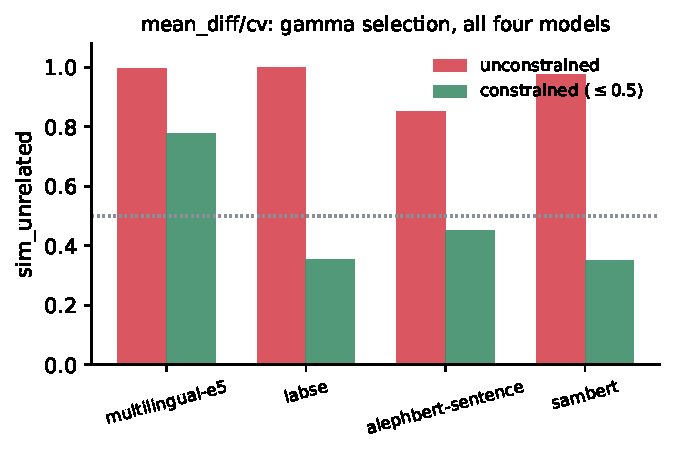
\includegraphics[width=0.5\textwidth]{fig_gamma_collapse.pdf}
\caption{Same phenomenon, all four models, mean-difference direction,
cross-validated selection: unconstrained selection lands on
$\mathrm{sim\_unrelated} \geq 0.85$ every time; the constrained version
lands under 0.45 on three of four (multilingual-e5 is the exception
discussed above).}
\label{fig:gammacollapse}
\end{figure}

\subsection{\texttt{nli\_rerank}: locked test-set numbers}

Our fine-tuned classifier reaches 79.6\% test accuracy (macro-F1 79.4\%) on
the clean HebNLI test split, against 72.7\% (macro-F1 72.2\%) for the
released \texttt{LCHAIM} checkpoint on the same split. This is not a fair
comparison, but not for the reason it might first appear: it is not fair
\emph{in the classifier's own favor}, since the released checkpoint was
fine-tuned on all of HebNLI rather than a held-out split, so this test set
was very likely part of its own training data --- a documented caveat on
that evaluation run. Contamination should inflate a model's score, not
deflate it, so the released checkpoint scoring seven points lower despite
that likely advantage is stronger evidence for training a task-specific
classifier than a same-objective comparison would have given us. The same
pattern holds directly on the probe task itself, not just generic HebNLI:
scoring both checkpoints with $\lambda=1$ (pure NLI, no cosine
contribution) on \texttt{multilingual-e5}'s probe pairs, our classifier
reaches 0.993 pairwise accuracy against LCHAIM's 0.987. Both classifiers'
weakest class is \emph{neutral}, but by different margins --- our
classifier's neutral recall is 0.740, LCHAIM's is 0.575, while LCHAIM
over-predicts \emph{contradiction} in its place.

\begin{table}[h]
\centering
\small
\begin{tabular}{lrrrr}
\toprule
model & $\lambda$ & pairwise acc.\ ($\lambda{=}0 \to$ selected) & STS Spearman ($\lambda{=}0 \to$ selected) & test drop \\
\midrule
multilingual-e5 & 0.05 & 0.80 $\to$ \textbf{0.99} & 0.76 $\to$ 0.76 & 0.007 \\
LaBSE & 0.35 & 0.79 $\to$ \textbf{0.99} & 0.74 $\to$ 0.67 & \textbf{0.070} \\
alephbert-sentence & 0.30 & 0.50 $\to$ \textbf{0.99} & 0.65 $\to$ 0.65 & 0.000 \\
sambert & 0.35 & 0.50 $\to$ \textbf{0.99} & 0.69 $\to$ 0.67 & 0.014 \\
\bottomrule
\end{tabular}
\caption{Every model reaches $\geq$0.986 pairwise accuracy. The 0.02
STS-Spearman-drop budget is a \emph{dev-time} selection criterion (see
Methodology); the rightmost column is what that drop actually turned out to
be on the locked \emph{test} split. Three of four models stay well inside
the dev-time budget (test drop $\leq$0.014). LaBSE does not: its dev-time
margin was already narrow (0.019 of the 0.02 budget), and that margin did
not survive contact with the held-out split --- its test-time drop is
$3.5\times$ the budget it was selected under. This is a real result about
the selection rule's generalization, not a rounding error, and is discussed
further in Limitations.}
\label{tab:nlirerank}
\end{table}

\begin{figure}[h]
\centering
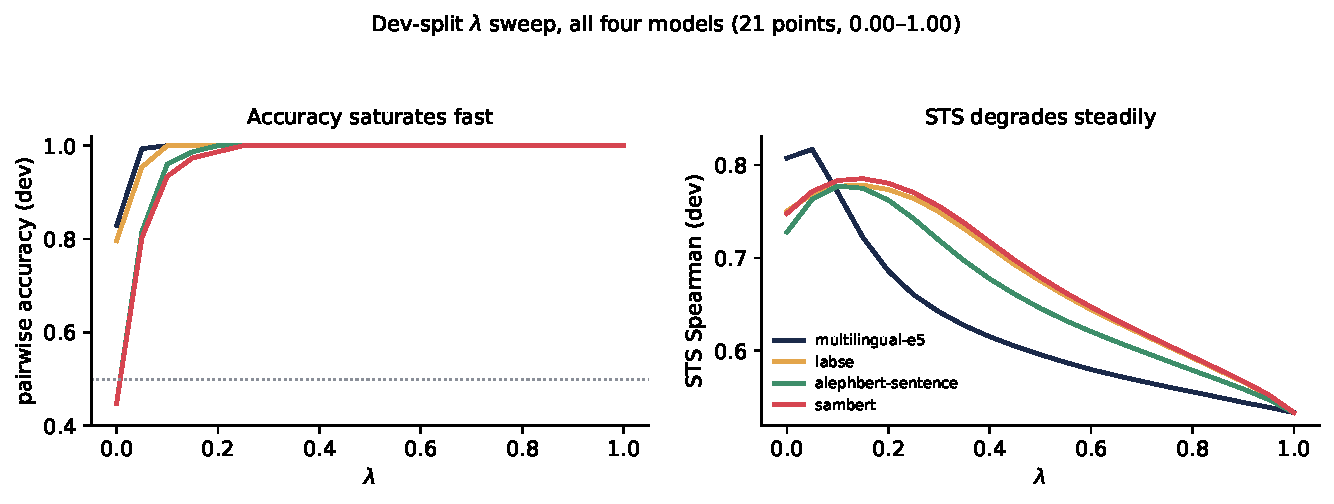
\includegraphics[width=0.78\textwidth]{fig_lambda_sweep.pdf}
\caption{Dev-split $\lambda$ sweep behind ``a small $\lambda$ is enough'':
pairwise accuracy saturates near $\lambda \approx 0.1$--0.2 for every
model, while STS Spearman rises slightly and then declines from there ---
the two curves justify why the selection rule finds a small $\lambda$
sufficient rather than needing to trade deep into the STS budget.}
\label{fig:lambdasweep}
\end{figure}

\subsection{Head-to-head}

\begin{table}[h]
\centering
\small
\begin{tabular}{llrl}
\toprule
model & intervention & pairwise acc.\ & trade-off guard \\
\midrule
\multirow{3}{*}{multilingual-e5}
 & baseline & 0.80 & STS 0.76 \\
 & projection (mean-diff, $\gamma$=12, relaxed) & 0.97 & sim\_unrel 0.78 (over budget) \\
 & nli\_rerank ($\lambda$=0.05) & \textbf{0.99} & STS 0.76 \\
\multirow{3}{*}{LaBSE}
 & baseline & 0.80 & STS 0.74 \\
 & projection (mean-diff, $\gamma$=5) & \textbf{0.99} & sim\_unrel 0.35 \\
 & nli\_rerank ($\lambda$=0.35) & \textbf{0.99} & STS 0.67 (0.070 test drop) \\
\multirow{3}{*}{alephbert-sentence}
 & baseline & 0.50 & STS 0.65 \\
 & projection (mean-diff, $\gamma$=12) & 0.97 & sim\_unrel 0.45 \\
 & nli\_rerank ($\lambda$=0.30) & \textbf{0.99} & STS 0.65 \\
\multirow{3}{*}{sambert}
 & baseline & 0.50 & STS 0.70 \\
 & projection (mean-diff, $\gamma$=12) & 0.88 & sim\_unrel 0.35 \\
 & nli\_rerank ($\lambda$=0.35) & \textbf{0.99} & STS 0.67 \\
\bottomrule
\end{tabular}
\caption{\texttt{projection}'s own default configuration (mean-difference
direction, centered, cross-validated $\gamma$), constrained to
$\mathrm{sim\_unrelated} \leq 0.5$, applied identically to all four models
--- not the best of the 8 direction/centering/selection combinations we
separately ablate (Section \ref{sec:results}), since picking per model
whichever of those scores highest on test would itself be test-set
selection (multilingual-e5: the constraint is unsatisfiable here, so the
lowest-\emph{sim\_unrelated} point is shown, flagged relaxed).
$\mathrm{sim\_unrelated}$ and STS are on different scales and not directly
comparable, so both guards are reported alongside rather than merged;
\texttt{nli\_rerank} wins on every model on accuracy, with a real
semantic-similarity guard rather than a proxy, except that its own guard
did not hold at test time for LaBSE (Table \ref{tab:nlirerank}).
\texttt{projection} needs no second model at inference time and closes
most of the accuracy gap on three of four models, sambert being the
exception.}
\label{tab:headtohead}
\end{table}

\subsection{Where the fixes still fail: per-category breakdown}

\begin{table}[h]
\centering
\small
\begin{tabular}{lrrrr}
\toprule
category & $n$ ($\times$4 models) & baseline pass rate & projection pass rate & gap closed \\
\midrule
particle (\heb{לא}) & 356 & 0.67 & 0.96 & 87\% \\
existential (\heb{אין}) & 100 & 0.65 & 0.95 & 86\% \\
quantifier & 108 & 0.61 & 0.94 & 86\% \\
question & 16 & 0.25 & 0.75 & 67\% \\
privative & 12 & 0.75 & 1.00 & 100\% \\
neg-raising & 12 & 0.83 & 1.00 & 100\% \\
\bottomrule
\end{tabular}
\caption{Per-category pass rate, aggregated across all four models,
baseline vs.\ \texttt{projection} (the same fixed default configuration as
Table \ref{tab:headtohead}, not a per-model best-of-8 pick).}
\label{tab:percategory}
\end{table}

The three largest categories --- particle, existential, quantifier,
together 89\% of the test items --- all see \texttt{projection} close
roughly 86--87\% of the baseline gap. \texttt{question} (16 items) recovers
the least in relative terms, 67\%, despite a mid-range starting point.
\texttt{privative} and \texttt{neg-raising} (12 items combined) each close
100\% of their gap, but at 3 items per model that is as plausibly a
small-$n$ ceiling effect as genuine ease --- the same low-$n$ caveat as
before, just cutting the other way: this reads as a real but uncertain
signal, not a confident claim that these categories are easiest.

\section{Discussion}

We confirmed the negation blind spot exists in Hebrew sentence embeddings
--- two of four frozen models score a sentence's negation as \emph{more}
similar to it than a faithful paraphrase --- and tested two ways to repair
it without retraining the embedder. \texttt{nli\_rerank} closes the gap
almost completely on every model ($\geq$0.986 pairwise accuracy) while a
semantic-similarity guard stays within its dev-time budget for three of
four models (Results; LaBSE is the exception). \texttt{projection}
recovers a substantial share of the gap without a second model at
inference time, but only once its own selection procedure is constrained
against a collapse guard.

\textbf{The methodological finding, not just the fix, is the contribution.}
The unconstrained-$\gamma$ failure mode fell out of widening the search
grid on real models and noticing the headline metric kept improving in a
direction that should have been suspicious. The contribution is that
amplifying a concept direction safely requires a second, independent guard
metric; that gap-only selection reliably finds the degenerate optimum
instead of the intended one; and that cross-validation does not protect
against this particular failure, because collapse improves the metric on
every fold, held out or not. \texttt{nli\_rerank}'s $\lambda$-selection
rule was built on the same principle independently (a hard STS budget, not
a weighted trade-off), and the two interventions validate each other on
this point.

\subsection{Limitations}

\begin{itemize}
\item \textbf{Probe size.} 303 items (151 test) is small; the smallest
per-category slices (3--4 items per model) are suggestive, not conclusive.
\item \textbf{$\mathrm{sim\_unrelated}$ is a proxy, not a real similarity
benchmark.} It is exactly what let \texttt{nli\_rerank}'s STS guard catch a
generalization failure (LaBSE, Table \ref{tab:nlirerank}) that
\texttt{projection}'s proxy guard has no way to catch, since it is only
measured on train via cross-validation and never checked against a held-out
split at all; \texttt{projection} would benefit from the same held-out
Hebrew-STS guard \texttt{nli\_rerank} already has, which we did not have
time to wire in.
\item \textbf{Hebrew STS-B is a translation} of the English benchmark
\citep{agirre2017semeval} with inherited English gold scores, not natively
annotated in Hebrew; machine-translated STS benchmarks are known to
introduce translation artifacts \citep{isbister2020swedish}, and our
two-translator-plus-adjudicator pipeline with a human spot-check reduces
but does not eliminate that risk.
\item \textbf{The 0.02 STS budget is a dev-time guarantee, not a test-time
one.} It held on test for three of four models but not LaBSE, whose
dev-time margin was already narrow (Table \ref{tab:nlirerank}) --- a
budget checked once on dev does not certify every model's behavior on
unseen data.
\item \textbf{No $\gamma$ in our search grid resolves \texttt{multilingual-e5}'s}
collapse guard.
\item \textbf{Single-run test evaluation.} Each configuration is evaluated
once on the locked test split rather than averaged over seeds, appropriate
for the ``no peeking'' guarantee but meaning we cannot separately quantify
the variance in any single reported number.
\end{itemize}

\subsection{Future work}

Wire a held-out Hebrew STS guard into \texttt{projection}'s
$\gamma$-selection, matching \texttt{nli\_rerank}'s dev/test discipline.
Extend the probe with a fourth sentence per item to enable a true
NevIR-style 0.25-chance metric. Investigate why \texttt{multilingual-e5}
resists the collapse-safe region entirely, and why LaBSE's STS margin does
not generalize from dev to test while the other three models' do.

\section{Code}

Full code, data, and results:
\url{https://github.com/ItayBoros/hebrew-negation-embeddings} (branch
\texttt{main}). Colab notebooks for the GPU-dependent stages (probe mining,
real-model evaluation, NLI fine-tuning, $\lambda$ selection) are under
\texttt{notebooks/}.

\bibliographystyle{plainnat}
\bibliography{references}

\end{document}
